\documentclass[11pt,a4paper]{article}

% =============================================================================
% PACKAGES
% =============================================================================
\usepackage[utf8]{inputenc}
\usepackage[T1]{fontenc}
\usepackage[french]{babel}
\usepackage{amsmath}
\usepackage{lmodern}
\usepackage[margin=2.2cm, headheight=15pt]{geometry}
\usepackage{graphicx}
\usepackage{xcolor}
\usepackage{booktabs}
\usepackage{tabularx}
\usepackage{array}
\usepackage{float}
\usepackage{enumitem}
\usepackage{fancyhdr}
\usepackage{titlesec}
\usepackage{tcolorbox}
\usepackage{tikz}
\usetikzlibrary{shapes.geometric, arrows.meta, positioning, fit, backgrounds, calc}
\usepackage[colorlinks=true, linkcolor=inseaBlue, urlcolor=inseaTeal, citecolor=inseaBlue, plainpages=false, pdfpagelabels]{hyperref}

% =============================================================================
% COULEURS & STYLES
% =============================================================================
\definecolor{inseaBlue}{HTML}{1B365D}
\definecolor{inseaTeal}{HTML}{0E7490}
\definecolor{inseaLight}{HTML}{F0F4F8}
\definecolor{stdBg}{HTML}{EFF6FF}
\definecolor{stdBorder}{HTML}{2563EB}
\definecolor{extBg}{HTML}{FFFBEB}
\definecolor{extBorder}{HTML}{D97706}
\definecolor{customBg}{HTML}{ECFDF5}
\definecolor{customBorder}{HTML}{059669}
\definecolor{refuseBg}{HTML}{FEF2F2}
\definecolor{refuseBorder}{HTML}{DC2626}
\definecolor{grayText}{HTML}{475569}

\titleformat{\section}
  {\Large\bfseries\color{inseaBlue}}{\thesection}{0.8em}{}[\vspace{2pt}\titlerule]
\titleformat{\subsection}
  {\large\bfseries\color{inseaTeal}}{\thesubsection}{0.7em}{}
\titleformat{\subsubsection}
  {\normalsize\bfseries\color{inseaBlue}}{\thesubsubsection}{0.6em}{}

\pagestyle{fancy}
\fancyhf{}
\fancyhead[L]{\small\color{grayText} INSEA -- 2\textsuperscript{ème} Année Master M2SI \quad|\quad Systèmes Intégrés (Odoo 18)}
\fancyhead[R]{\small\color{grayText} Module \texttt{insea\_hr\_leave\_custom}}
\fancyfoot[C]{\small\color{grayText}\thepage}
\renewcommand{\headrulewidth}{0.4pt}

\tcbset{
  infobox/.style={
    colback=inseaLight,
    colframe=inseaBlue,
    boxrule=0.8pt,
    arc=3pt,
    left=8pt, right=8pt, top=6pt, bottom=6pt,
    fonttitle=\bfseries\color{white},
    colbacktitle=inseaBlue
  }
}

\newcolumntype{Y}{>{\raggedright\arraybackslash}X}

% =============================================================================
% DOCUMENT
% =============================================================================
\begin{document}

% -----------------------------------------------------------------------------
% PAGE DE GARDE
% -----------------------------------------------------------------------------
\begin{titlepage}
    \centering
    \vspace*{0.5cm}
    {\large\bfseries\color{inseaBlue} ROYAUME DU MAROC}\\[0.2cm]
    {\Large\bfseries\color{inseaBlue} INSTITUT NATIONAL DE STATISTIQUE ET D'ÉCONOMIE APPLIQUÉE}\\[0.15cm]
    {\normalsize\color{grayText} (INSEA -- Rabat)}\\[0.6cm]
    \rule{\textwidth}{1.2pt}\\[0.3cm]
    {\large\bfseries Cycle Master : M2SI (2\textsuperscript{ème} Année)}\\[0.15cm]
    {\normalsize Module : Systèmes Intégrés (ERP) \quad---\quad Année Universitaire 2026 -- 2027}\\[0.3cm]
    \rule{\textwidth}{1.2pt}

    \vspace{2.2cm}
    \begin{tcolorbox}[colback=inseaLight, colframe=inseaBlue, boxrule=1.5pt, arc=6pt,
                      top=18pt, bottom=18pt, left=14pt, right=14pt]
        \centering
        {\small\scshape\color{inseaTeal} Rapport de Mini-Projet Systèmes Intégrés}\\[0.4cm]
        {\LARGE\bfseries\color{inseaBlue} Mise en place d'une solution intégrée de gestion des autorisations d'absence et des congés (RH)}\\[0.5cm]
        {\large\color{grayText} Conception UML, développement et validation du module Odoo 18 \texttt{insea\_hr\_leave\_custom}}
    \end{tcolorbox}

    \vspace{2.2cm}
    \begin{center}
        {\large\bfseries\color{inseaBlue} Réalisé par :}\\[0.35cm]
        {\large Yahya \textsc{Ghallali}}\\[0.15cm]
        {\large Mohamed \textsc{Eddaoudi}}\\[0.25cm]
        {\normalsize\color{grayText} 2\textsuperscript{ème} Année Cycle Master M2SI -- INSEA Rabat}
    \end{center}

    \vfill
    {\normalsize\color{grayText} Année Universitaire 2026 -- 2027}
\end{titlepage}

\tableofcontents
\newpage

% =============================================================================
% 1. CONTEXTE ET EXPRESSION DES BESOINS
% =============================================================================
\section{Contexte et Expression des Besoins}

\subsection{Problématique métier}
Dans le cadre de la modernisation de ses processus RH et de la dématérialisation de ses circuits administratifs, la société \textbf{Lambda} souhaite déployer un module dédié sous l'ERP open-source \textbf{Odoo}. Jusqu'à présent, la gestion des absences de courte durée et des congés légaux reposait sur des formulaires papier et des échanges informels, engendrant :
\begin{itemize}[itemsep=2pt]
    \item des retards dans le circuit de validation hiérarchique et RH ;
    \item des erreurs de décompte dans le solde des congés payés annuels ;
    \item un manque de visibilité des managers opérationnels lors de la planification des équipes.
\end{itemize}

L'objectif du mini-projet est de concevoir, développer et valider un module Odoo personnalisé (\texttt{insea\_hr\_leave\_custom}) garantissant l'application stricte des règles métier, la traçabilité complète des décisions et une isolation rigoureuse des données selon le profil utilisateur.

\subsection{Spécifications fonctionnelles}
Le module couvre deux volets complémentaires résumés dans le tableau~\ref{tab:specs}.

\begin{table}[H]
\centering
\caption{Synthèse des catégories de demandes et de leurs règles métier}
\label{tab:specs}
\small
\begin{tabularx}{\textwidth}{>{\bfseries}p{3.4cm} Y Y}
\toprule
Catégorie & Caractéristiques \& limites & Impact solde \& justificatif \\
\midrule
Autorisation de sortie (courte durée) &
Durée en heures ($\leq 4\text{ h}$, soit une demi-journée). Plafonnée à \textbf{3 autorisations} ou \textbf{8 heures cumulées} par mois calendaire. Motif obligatoire (consultation médicale, démarche administrative, urgence personnelle). &
N'impacte pas le solde de congés payés. Justificatif (PDF/image) obligatoire pour le motif \textit{consultation médicale}. \\
\midrule
Congé payé annuel &
Décompté en jours ouvrés (lundi à vendredi, hors jours fériés). Délai de prévenance de \textbf{7 jours calendaires} si durée $> 3\text{ jours}$. &
Acquisition de \textbf{1,5 jour / mois} de travail effectif. Déduction automatique après validation RH. \\
\midrule
Congé exceptionnel (événement familial) &
Durées réglementaires : \textbf{mariage (4 j)}, \textbf{naissance (3 j)}, \textbf{décès (2 à 3 j)}. Date de fin pré-remplie automatiquement. &
N'impacte pas le solde de congés payés. Justificatif obligatoire (acte d'état civil). \\
\midrule
Congé maladie ordinaire &
Décompté en jours ouvrés. Si durée $= 1\text{ j}$, validation finale par le manager N+1 ; si $> 1\text{ j}$, validation RH requise. &
N'impacte pas le solde de congés payés. Certificat médical obligatoire avant validation finale. \\
\bottomrule
\end{tabularx}
\end{table}

\subsection{Contrôles d'intégrité et circuit de validation}
Quatre contrôles d'intégrité transverses s'appliquent automatiquement :
\begin{enumerate}[itemsep=2pt]
    \item \textbf{Disponibilité du solde :} le solde disponible (acquis + report $-$ pris $-$ demandes payées en attente) doit être $\geq$ à la durée demandée lors de la soumission et de la validation RH.
    \item \textbf{Non-chevauchement :} interdiction absolue de saisir une demande chevauchant une autre demande active (\textit{Soumis}, \textit{Validé N+1} ou \textit{Validé}) pour le même collaborateur, quelle que soit la catégorie.
    \item \textbf{Délai de prévenance :} tout congé payé strictement supérieur à 3 jours ouvrés doit être soumis au moins 7 jours calendaires avant la date de début.
    \item \textbf{Blocage sur justificatif manquant :} la validation finale (manager ou RH selon le cas) est bloquée tant qu'aucune pièce jointe n'est associée aux demandes qui l'exigent.
\end{enumerate}

Les demandes suivent un cycle de vie en 5 états (\textit{Brouillon}, \textit{Soumis}, \textit{Validé N+1}, \textit{Validé}, \textit{Refusé}). Après soumission, la demande est verrouillée en écriture pour l'employé (hormis l'ajout de pièces justificatives tant qu'elle est en cours d'instruction). Tout refus impose la saisie d'un motif et notifie automatiquement l'employé dans le fil de discussion (\textit{chatter}).

% =============================================================================
% 2. CONCEPTION ET ARCHITECTURE LOGICIELLE (UML)
% =============================================================================
\section{Conception et Architecture Logicielle (UML)}

\subsection{Diagramme de Cas d'Utilisation}
Le diagramme de cas d'utilisation (figure~\ref{fig:usecase}) modélise les quatre acteurs du système : \textbf{Employé}, \textbf{Responsable Hiérarchique (Manager N+1)}, \textbf{Responsable RH} et \textbf{Administrateur Système}. L'héritage entre acteurs reflète la hiérarchie des groupes Odoo : un Manager dispose des droits d'un Employé, et un Responsable RH hérite des droits du Manager.

\begin{figure}[H]
\centering
\begin{tikzpicture}[
    scale=0.88, transform shape,
    actor/.style={draw=inseaBlue, fill=inseaLight, rounded corners=3pt, minimum width=2.7cm, minimum height=0.85cm, align=center, font=\small\bfseries\color{inseaBlue}},
    uc/.style={ellipse, draw=inseaTeal, fill=white, minimum width=3.8cm, minimum height=0.78cm, align=center, font=\footnotesize},
    assoc/.style={-{Stealth[length=2.2mm]}, thick, color=inseaBlue!80},
    inh/.style={-{Triangle[open, length=3mm, width=2.5mm]}, thick, color=inseaBlue},
    inc/.style={-{Stealth[length=2mm]}, dashed, color=grayText}
]
    % System boundary
    \draw[rounded corners=8pt, draw=inseaBlue, fill=inseaLight!35, thick] (2.4, -7.8) rectangle (14.4, 3.6);
    \node[anchor=north west, font=\small\bfseries\color{inseaBlue}] at (2.6, 3.45) {Système Odoo -- Module \texttt{insea\_hr\_leave\_custom}};

    % Actors
    \node[actor] (emp) at (0, 2.0) {Employé};
    \node[actor] (mgr) at (0, -1.2) {Manager (N+1)};
    \node[actor] (hr)  at (0, -4.4) {Responsable RH};
    \node[actor] (adm) at (0, -6.9) {Admin. Système};

    % Actor inheritance
    \draw[inh] (mgr.north) -- (emp.south);
    \draw[inh] (hr.north) -- (mgr.south);
    \draw[inh] (adm.north) -- (hr.south);

    % Use cases - Employee
    \node[uc] (uc1) at (6.0, 2.4) {Créer / soumettre\\une demande};
    \node[uc] (uc2) at (11.7, 2.4) {Joindre un justificatif\\(PDF / image)};
    \node[uc] (uc3) at (6.0, 0.9) {Consulter ses demandes\\et son solde};

    % Use cases - Manager
    \node[uc] (uc4) at (6.0, -0.8) {Valider (N+1) les\\demandes de l'équipe};
    \node[uc] (uc5) at (11.7, -1.6) {Refuser une demande\\avec motif obligatoire};
    \node[uc] (uc6) at (6.0, -2.3) {Consulter le planning\\calendrier d'équipe};

    % Use cases - HR
    \node[uc] (uc7) at (6.0, -4.1) {Effectuer la validation\\finale RH};
    \node[uc] (uc8) at (11.7, -4.1) {Consulter les analyses\\(Graphique / Pivot)};
    \node[uc] (uc9) at (6.0, -5.6) {Gérer soldes, reports\\et jours fériés};

    % Use cases - Admin
    \node[uc] (uc10) at (11.7, -6.8) {Gérer utilisateurs,\\groupes et règles d'accès};

    % Associations
    \draw[assoc] (emp.east) -- (uc1.west);
    \draw[assoc] (emp.east) -- (uc3.west);
    \draw[assoc] (mgr.east) -- (uc4.west);
    \draw[assoc] (mgr.east) -- (uc6.west);
    \draw[assoc] (hr.east) -- (uc7.west);
    \draw[assoc] (hr.east) -- (uc9.west);
    \draw[assoc] (hr.east) -- (uc8.west);
    \draw[assoc] (adm.east) -- (uc10.west);

    % Include / Extend
    \draw[inc] (uc1.east) -- node[above, font=\scriptsize\itshape] {$\ll$extend$\gg$} (uc2.west);
    \draw[inc] (uc4.east) -- node[above, font=\scriptsize\itshape, sloped] {$\ll$extend$\gg$} (uc5.west);
    \draw[inc] (uc7.east) -- node[below, font=\scriptsize\itshape, sloped] {$\ll$extend$\gg$} (uc5.south west);
\end{tikzpicture}
\caption{Diagramme de Cas d'Utilisation du module \texttt{insea\_hr\_leave\_custom}}
\label{fig:usecase}
\end{figure}

\subsection{Diagramme de Classes UML (Classes Standard vs. Sur-Mesure)}
Conformément au cahier des charges, la figure~\ref{fig:classdiag} distingue visuellement et sémantiquement trois niveaux d'architecture Odoo :
\begin{itemize}[itemsep=1pt]
    \item \textbf{\color{stdBorder} Bleu (pointillé) -- Classes standard Odoo réutilisées} : \texttt{res.users}, \texttt{hr.department}, \texttt{ir.attachment}, \texttt{mail.thread / mail.activity.mixin}, \texttt{resource.calendar.leaves}.
    \item \textbf{\color{extBorder} Ambre -- Classe standard étendue par héritage (\texttt{\_inherit})} : \texttt{hr.employee}.
    \item \textbf{\color{customBorder} Vert -- Classes créées sur-mesure (\texttt{\_name})} : le modèle métier principal \texttt{insea.absence.request} et le modèle transitoire \texttt{insea.absence.refuse.wizard}.
\end{itemize}

\begin{figure}[H]
\centering
\begin{tikzpicture}[
    scale=0.72, transform shape,
    std/.style={rectangle, draw=stdBorder, dashed, line width=1pt, fill=stdBg, rounded corners=2pt, text width=4.3cm, align=left, font=\scriptsize, inner sep=5pt},
    ext/.style={rectangle, draw=extBorder, line width=1.2pt, fill=extBg, rounded corners=2pt, text width=5.1cm, align=left, font=\scriptsize, inner sep=5pt},
    custom/.style={rectangle, draw=customBorder, line width=1.2pt, fill=customBg, rounded corners=2pt, text width=6.1cm, align=left, font=\scriptsize, inner sep=5pt},
    assoc/.style={-{Stealth[length=2.2mm]}, thick, color=inseaBlue!85},
    inh/.style={-{Triangle[open, length=3mm, width=2.4mm]}, thick, color=stdBorder}
]
    % Standard mixins (top)
    \node[std, text width=5.4cm] (mail) at (0.4, 6.2) {
        \centering\textbf{\color{stdBorder}$\ll$Odoo Standard Mixin$\gg$}\\
        \textbf{mail.thread \& mail.activity.mixin}\\[2pt]
        \hrule\vspace{2pt}
        \raggedright
        + message\_ids, activity\_ids\\
        + message\_post(), activity\_schedule()
    };

    % Standard res.users
    \node[std] (users) at (-7.4, 3.6) {
        \centering\textbf{\color{stdBorder}$\ll$Odoo Standard$\gg$}\\
        \textbf{res.users}\\[2pt]
        \hrule\vspace{2pt}
        \raggedright
        + login, name, tz\\
        + groups\_id (M2M)
    };

    % Standard hr.department
    \node[std] (dept) at (-7.4, 0.7) {
        \centering\textbf{\color{stdBorder}$\ll$Odoo Standard$\gg$}\\
        \textbf{hr.department}\\[2pt]
        \hrule\vspace{2pt}
        \raggedright
        + name : Char
    };

    % Extended hr.employee
    \node[ext] (emp) at (-7.0, -3.2) {
        \centering\textbf{\color{extBorder}$\ll$\_inherit = 'hr.employee'$\gg$}\\
        \textbf{HrEmployee (Extension)}\\[2pt]
        \hrule\vspace{2pt}
        \raggedright
        + insea\_hire\_date : Date\\
        + insea\_initial\_balance : Float\\
        + insea\_months\_worked : Integer (calc.)\\
        + insea\_leave\_accrued : Float (calc.)\\
        + insea\_leave\_taken : Float (calc.)\\
        + insea\_leave\_pending : Float (calc.)\\
        + insea\_leave\_balance : Float (calc.)\\
        \hrule\vspace{2pt}
        + \_compute\_leave\_balance()\\
        + action\_open\_insea\_requests()
    };

    % Custom insea.absence.request
    \node[custom] (req) at (0.4, 0.0) {
        \centering\textbf{\color{customBorder}$\ll$\_name = 'insea.absence.request'$\gg$}\\
        \textbf{InseaAbsenceRequest (Nouveau modèle)}\\[2pt]
        \hrule\vspace{2pt}
        \raggedright
        + name : Char (séquence \texttt{ABS/YYYY/00001})\\
        + category : Selection (auth/paid/exceptional/sick)\\
        + authorization\_reason, authorization\_date\\
        + hour\_from, hour\_to : Float\\
        + family\_event, date\_from, date\_to\\
        + start\_datetime, end\_datetime : Datetime (calc.)\\
        + duration\_hours, duration\_days : Float (calc.)\\
        + requires\_attachment, requires\_hr\_validation : Bool\\
        + state : Selection (5 états)\\
        + manager\_user\_id, hr\_user\_id, refusal\_reason\\
        \hrule\vspace{2pt}
        + \_check\_authorization\_duration() / \_monthly\_cap()\\
        + \_check\_overlap(), \_check\_balance(), \_check\_notice\_period()\\
        + action\_submit(), action\_manager\_approve()\\
        + action\_hr\_approve(), \_do\_refuse(), action\_reset\_to\_draft()\\
        + write(), unlink() \textit{(verrouillage post-soumission)}
    };

    % Standard ir.attachment
    \node[std] (att) at (8.1, 3.0) {
        \centering\textbf{\color{stdBorder}$\ll$Odoo Standard$\gg$}\\
        \textbf{ir.attachment}\\[2pt]
        \hrule\vspace{2pt}
        \raggedright
        + name, datas, mimetype\\
        + res\_model, res\_id
    };

    % Standard resource.calendar.leaves
    \node[std] (hol) at (8.1, 0.0) {
        \centering\textbf{\color{stdBorder}$\ll$Odoo Standard$\gg$}\\
        \textbf{resource.calendar.leaves}\\[2pt]
        \hrule\vspace{2pt}
        \raggedright
        + name, date\_from, date\_to\\
        + calendar\_id (jours fériés)
    };

    % Custom TransientModel Wizard
    \node[custom, text width=4.6cm] (wiz) at (8.1, -3.2) {
        \centering\textbf{\color{customBorder}$\ll$TransientModel$\gg$}\\
        \textbf{insea.absence.refuse.wizard}\\[2pt]
        \hrule\vspace{2pt}
        \raggedright
        + request\_id : Many2one\\
        + reason : Text (obligatoire)\\
        \hrule\vspace{2pt}
        + action\_confirm()
    };

    % Relations
    \draw[inh] (req.north) -- (mail.south);
    \draw[assoc] (req.west) -- ++(-0.7,0) |- node[pos=0.72, above, font=\scriptsize, fill=white, inner sep=1pt] {employee\_id (N:1)} (emp.east);
    \draw[assoc] (emp.north) -- ++(0,0.4) -| node[pos=0.25, left, font=\scriptsize] {department\_id} (dept.south);
    \draw[assoc] (users.south east) -- node[right, font=\scriptsize] {user\_id} (emp.north east);
    \draw[assoc] (req.east) -- ++(0.6,0) |- node[pos=0.72, above, font=\scriptsize, fill=white, inner sep=1pt] {attachment\_ids} (att.west);
    \draw[assoc, dashed] (req.east) -- node[above, font=\scriptsize] {consulte} (hol.west);
    \draw[assoc] (wiz.west) -- ++(-0.6,0) |- node[pos=0.72, below, font=\scriptsize, fill=white, inner sep=1pt] {request\_id} (req.south east);
\end{tikzpicture}
\caption{Diagramme de Classes UML distinguant les classes Odoo standard, étendues (\texttt{\_inherit}) et sur-mesure (\texttt{\_name})}
\label{fig:classdiag}
\end{figure}

\subsection{Diagramme d'États-Transitions}
La figure~\ref{fig:statediag} présente la machine à états complète d'une instance \texttt{insea.absence.request}, incluant les gardes métier vérifiées à chaque transition.

\begin{figure}[H]
\centering
\begin{tikzpicture}[
    scale=0.80, transform shape,
    state/.style={rectangle, rounded corners=8pt, draw=inseaBlue, fill=inseaLight, line width=1pt, minimum width=2.9cm, minimum height=1.05cm, align=center, font=\small\bfseries, text=inseaBlue},
    approved/.style={state, draw=customBorder, fill=customBg, text=customBorder},
    refused/.style={state, draw=refuseBorder, fill=refuseBg, text=refuseBorder},
    trans/.style={-{Stealth[length=2.4mm]}, thick, color=inseaBlue},
    lbl/.style={font=\scriptsize, align=center, fill=white, inner sep=2pt}
]
    \node[circle, fill=inseaBlue, inner sep=3.5pt] (init) at (0, 0) {};
    \node[state] (draft) at (2.4, 0) {Brouillon\\(\texttt{draft})};
    \node[state] (sub) at (7.8, 0) {Soumis\\(\texttt{submitted})};
    \node[state] (mgr) at (14.0, 0) {Validé N+1\\(\texttt{manager\_approved})};
    \node[approved] (app) at (14.0, -4.4) {Validé\\(\texttt{approved})};
    \node[refused] (ref) at (7.8, -4.4) {Refusé\\(\texttt{refused})};

    % Transitions
    \draw[trans] (init) -- (draft);
    \draw[trans] (draft) -- node[lbl, above=3pt] {\texttt{action\_submit()}\\ \textit{[prévenance \& solde OK]}} (sub);

    \draw[trans] (sub) -- node[lbl, above=3pt] {\texttt{action\_manager\_approve()}\\ \textit{[validation RH requise]}} (mgr);

    \draw[trans] (sub.south east) to[out=-25, in=155] node[lbl, pos=0.45, above=3pt, sloped] {\texttt{action\_manager\_approve()}\\ \textit{[autoris. / mal. 1 j \& justif.]}} (app.north west);

    \draw[trans] (mgr) -- node[lbl, right=4pt] {\texttt{action\_hr\_approve()}\\ \textit{[justif. \& solde OK]}} (app);

    \draw[trans] (sub) -- node[lbl, left=4pt] {Refus N+1\\ \textit{[motif oblig.]}} (ref);

    \draw[trans] (mgr.south west) to[out=-145, in=25] node[lbl, pos=0.62, below=3pt, sloped] {Refus RH \textit{[motif oblig.]}} (ref.north east);

    \draw[trans] (ref.west) -| node[lbl, pos=0.25, below=3pt] {\texttt{action\_reset\_to\_draft()}\\ \textit{(reprise par l'employé)}} (draft.south);
\end{tikzpicture}
\caption{Diagramme d'États-Transitions d'une demande d'absence}
\label{fig:statediag}
\end{figure}

% =============================================================================
% 3. CHOIX D'IMPLÉMENTATION SOUS ODOO 18
% =============================================================================
\section{Choix d'Implémentation sous Odoo 18}

\subsection{Architecture du module \texttt{insea\_hr\_leave\_custom}}
Le module est structuré selon les bonnes pratiques Odoo 18 (tableau~\ref{tab:arch}). Il dépend uniquement des modules standard \texttt{hr} et \texttt{mail}, garantissant un déploiement léger et autonome.

\begin{table}[H]
\centering
\caption{Organisation par couches du module \texttt{insea\_hr\_leave\_custom}}
\label{tab:arch}
\small
\begin{tabularx}{\textwidth}{>{\bfseries}p{2.3cm} >{\raggedright\arraybackslash\footnotesize}p{5.5cm} Y}
\toprule
Couche & Fichier(s) & Responsabilité \\
\midrule
Squelette & \texttt{\_\_manifest\_\_.py}, \texttt{\_\_init\_\_.py} & Déclaration du module, dépendances (\texttt{hr}, \texttt{mail}), ordre de chargement XML/CSV. \\
Modèles & \texttt{models/hr\_employee.py} & Extension (\texttt{\_inherit}) de \texttt{hr.employee} : date d'embauche, report, compteurs calculés. \\
 & \texttt{models/absence\_request.py} & Modèle \texttt{insea.absence.request} : champs, calculs, contraintes Python/SQL, workflow, verrouillage CRUD. \\
Assistant & \texttt{wizard/refuse\_wizard.py} & \texttt{TransientModel} imposant un motif lors d'un refus. \\
Sécurité & \texttt{security/security.xml}, \texttt{ir.model.access.csv} & 3 groupes hiérarchiques, droits CRUD et 4 règles d'enregistrement (\texttt{ir.rule}). \\
Interfaces XML & \texttt{views/absence\_request\_views.xml}, \texttt{hr\_employee\_views.xml}, \texttt{menus.xml} & Vues Formulaire (statusbar, rubans, alertes), Liste, Recherche, Calendrier, Graphique, Pivot, onglet fiche employé, menus par rôle. \\
Données \& Tests & \texttt{data/ir\_sequence\_data.xml}, \texttt{demo/demo\_data.xml}, \texttt{tests/test\_absence\_request.py} & Séquence \texttt{ABS/2026/00001}, jeu de démonstration (5 profils, 7 demandes) et 25 tests automatisés. \\
\bottomrule
\end{tabularx}
\end{table}

\subsection{Justifications techniques clés}
\begin{itemize}[itemsep=3pt]
    \item \textbf{Modèle dédié plutôt que surcharge de \texttt{hr.leave} :} le module natif \texttt{hr.leave} impose sa propre machine à états (\texttt{confirm/validate1/validate}) et un système d'allocations distinct. Un modèle dédié \texttt{insea.absence.request} permet d'implémenter proprement les autorisations en heures avec plafonds mensuels, le solde calculé sur la date d'embauche et le workflow exact du cahier des charges, tout en réutilisant \texttt{hr.employee}, \texttt{ir.attachment}, \texttt{mail.thread} et \texttt{resource.calendar.leaves}.
    \item \textbf{Unification des 4 catégories :} le champ \texttt{category} regroupe les autorisations et les congés au sein d'une même classe. Les champs calculés \texttt{start\_datetime} et \texttt{end\_datetime} (convertis en UTC selon le fuseau \texttt{Africa/Casablanca}) permettent un contrôle unique de non-chevauchement et une vue Calendrier consolidée.
    \item \textbf{Solde calculé à la volée (non stocké) :} l'acquisition dépendant de la date du jour ($1{,}5\text{ j} \times \text{mois complets}$), le calcul dynamique via \texttt{@api.depends} garantit un solde toujours exact sans nécessiter de tâche planifiée (\texttt{ir.cron}). Les congés payés en attente sont réservés lors de la vérification du solde pour empêcher toute double soumission frauduleuse.
    \item \textbf{Intégrité et anti-contournement :} trois contraintes PostgreSQL (\texttt{\_sql\_constraints}) garantissent l'ordre des dates et la plage horaire $[0\text{ h}, 24\text{ h}]$. La surcharge de \texttt{write()} et \texttt{unlink()} interdit à l'employé de modifier ou supprimer une demande soumise, ainsi que de forcer le champ \texttt{state} hors des boutons métier (protégés par le contexte \texttt{insea\_workflow=True}). L'auto-validation par un manager sur sa propre demande est bloquée (\texttt{not own}).
\end{itemize}

\subsection{Politique de sécurité et droits d'accès}
La sécurité repose sur trois groupes hiérarchiques rattachés à la catégorie \textit{Absences \& Congés} :
\begin{enumerate}[itemsep=2pt]
    \item \textbf{Employé (\texttt{group\_absence\_employee})} : attribué à tout utilisateur interne.\\
    Règle : \texttt{[('employee\_id.user\_id', '=', user.id)]} -- accès strictement limité à ses propres demandes.
    \item \textbf{Responsable hiérarchique (\texttt{group\_absence\_manager})} : hérite d'Employé.\\
    Règle additionnelle : \texttt{[('employee\_id.parent\_id.user\_id', '=', user.id)]} -- accès aux demandes de son équipe directe (sans droit de suppression).
    \item \textbf{Responsable RH (\texttt{group\_absence\_hr})} : hérite de Manager et \texttt{hr.group\_hr\_user}.\\
    Règle : \texttt{[(1, '=', 1)]} -- accès global, validation finale, analyses et gestion des soldes.
\end{enumerate}

% =============================================================================
% 4. DÉMONSTRATION FONCTIONNELLE ET INTERFACES UTILISATEUR
% =============================================================================
\section{Démonstration Fonctionnelle et Interfaces Utilisateur}

\subsection{Jeu de données de démonstration}
L'application a été déployée dans un environnement Docker isolé (\texttt{postgres:16} + \texttt{odoo:18.0}) sur une base fraîche \texttt{insea\_db} chargée avec les cinq profils représentatifs du tableau~\ref{tab:demo}.

\begin{table}[H]
\centering
\caption{Comptes de démonstration configurés dans \texttt{demo/demo\_data.xml}}
\label{tab:demo}
\small
\begin{tabularx}{\textwidth}{p{2.2cm} p{2.8cm} p{3.6cm} Y}
\toprule
\textbf{Login / MDP} & \textbf{Collaborateur} & \textbf{Rôle Odoo} & \textbf{Contexte de démonstration} \\
\midrule
\texttt{yahya} / \texttt{yahya} & Yahya G. & Responsable RH & Validation finale RH, accès global, soldes et analyses. \\
\texttt{mohamed} / \texttt{mohamed} & Mohamed D. & Manager (N+1) & Chef d'équipe Data ; valide les demandes de son équipe. \\
\texttt{oualid} / \texttt{oualid} & Oualid A. & Employé & 14 mois d'ancienneté (21 j acquis, 3 j pris, 5 j soumis). \\
\texttt{issalmou} / \texttt{issalmou} & Issalmou A. & Employé & Embauche récente (2 mois $\Rightarrow$ 3 j acquis) ; autorisation médicale sans justificatif. \\
\texttt{bilal} / \texttt{bilal} & Bilal E. & Employé & Congé maladie validé N+1 avec certificat PDF joint (\texttt{certificat\_medical\_bilal.pdf}) ; autorisation refusée. \\
\bottomrule
\end{tabularx}
\end{table}

\subsection{Parcours Employé (Oualid A.)}
Connecté avec le compte \texttt{oualid}, l'employé ne visualise que le menu \textit{Mes demandes} : les menus de validation, d'analyse et de configuration RH lui sont masqués (figure~\ref{fig:emp_list}). La vue liste affiche les badges colorés par statut et la présence éventuelle de justificatifs.

\begin{figure}[H]
    \centering
    \fbox{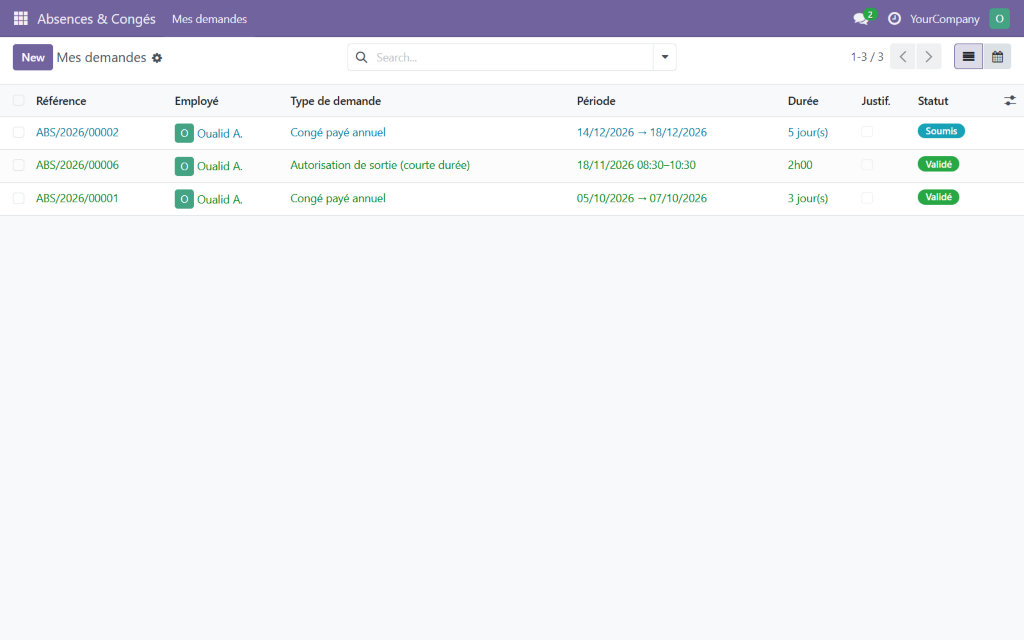
\includegraphics[width=0.95\textwidth]{figures/01_employee_list.png}}
    \caption{Vue liste \textit{Mes demandes} pour l'employé Oualid A. (isolation stricte des menus et enregistrements)}
    \label{fig:emp_list}
\end{figure}

L'ouverture de la demande \texttt{ABS/2026/00002} (figure~\ref{fig:emp_form}) met en évidence la barre de statut interactive (\texttt{statusbar}), le sélecteur de catégorie, le calcul automatique en jours ouvrés (\textit{5 jour(s)}), l'indicateur \textit{Validation RH requise} ainsi que le solde disponible (\textit{18,00 j}) et les jours en attente (\textit{5,00 j}).

\begin{figure}[H]
    \centering
    \fbox{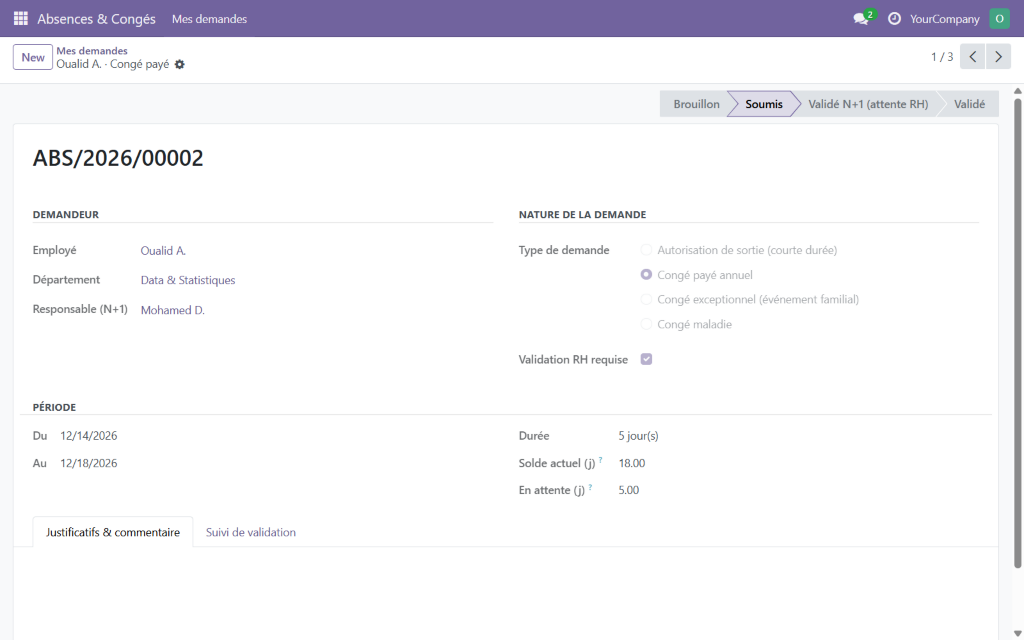
\includegraphics[width=0.95\textwidth]{figures/02_employee_form.png}}
    \caption{Formulaire de demande de congé payé soumis par Oualid A. (barre de statut et suivi du solde)}
    \label{fig:emp_form}
\end{figure}

\subsection{Parcours Manager N+1 (Mohamed D.)}
Le responsable hiérarchique \texttt{mohamed} accède aux menus \textit{Validation} (\textit{À valider (N+1)}, \textit{Toutes les demandes}) et \textit{Planning}. Sur une demande soumise par un membre de son équipe (figure~\ref{fig:mgr_val}), les boutons \textbf{Valider (N+1)} et \textbf{Refuser} (ouvrant l'assistant de saisie obligatoire du motif) sont activés.

\begin{figure}[H]
    \centering
    \fbox{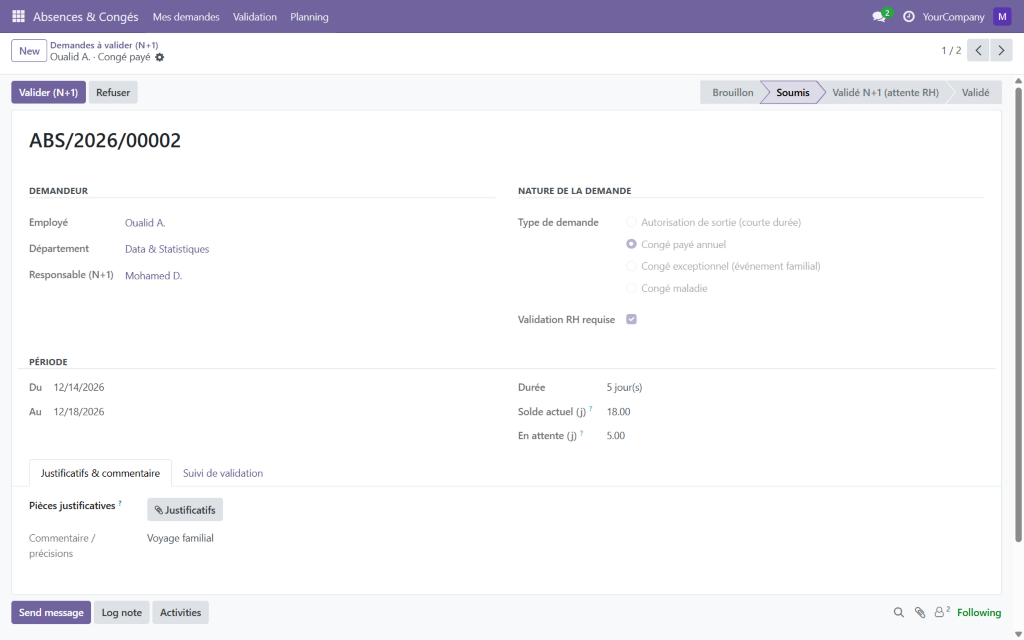
\includegraphics[width=0.95\textwidth]{figures/03_manager_validation.png}}
    \caption{Interface de validation N+1 pour le manager Mohamed D. sur la demande de Oualid A.}
    \label{fig:mgr_val}
\end{figure}

La vue \textbf{Planning} (figure~\ref{fig:mgr_cal}) offre au manager une visibilité mensuelle consolidée des congés et autorisations de son équipe, avec filtres latéraux par employé et par type de demande.

\begin{figure}[H]
    \centering
    \fbox{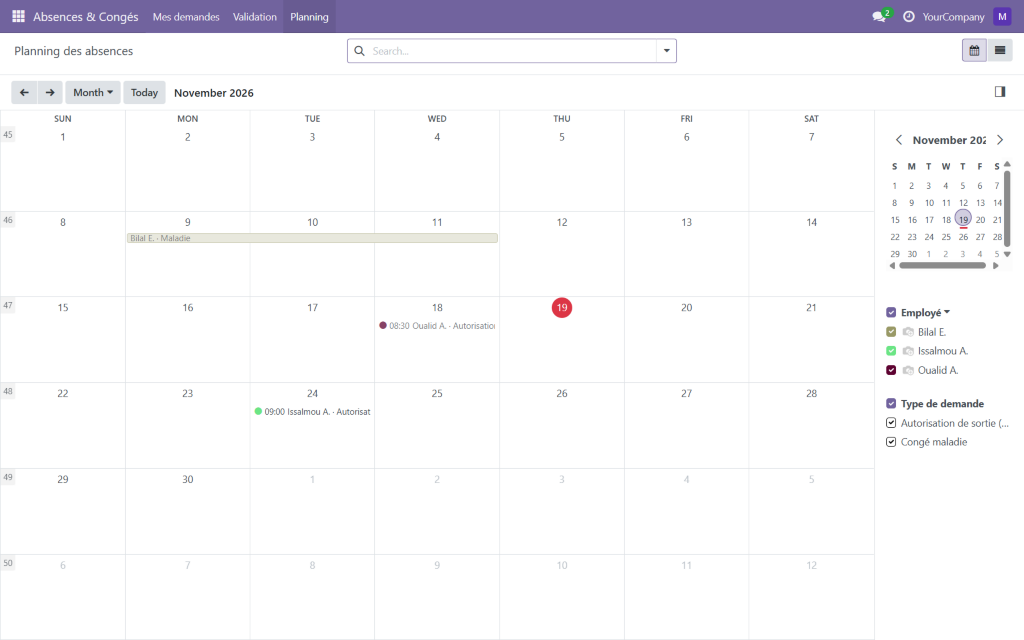
\includegraphics[width=0.95\textwidth]{figures/04_manager_calendar.png}}
    \caption{Vue Calendrier (\textit{Planning des absences}) accessible au manager Mohamed D.}
    \label{fig:mgr_cal}
\end{figure}

\subsection{Parcours Responsable RH (Yahya G.)}
Le Responsable RH \texttt{yahya} dispose de l'ensemble des menus, y compris \textit{Validation RH}, \textit{Analyse} et \textit{Configuration}. La figure~\ref{fig:hr_val} illustre la validation finale du congé maladie de Bilal E. (\texttt{ABS/2026/00004}), déjà approuvé par son N+1 et accompagné du certificat médical \texttt{certificat\_medical\_bilal.pdf}.

\begin{figure}[H]
    \centering
    \fbox{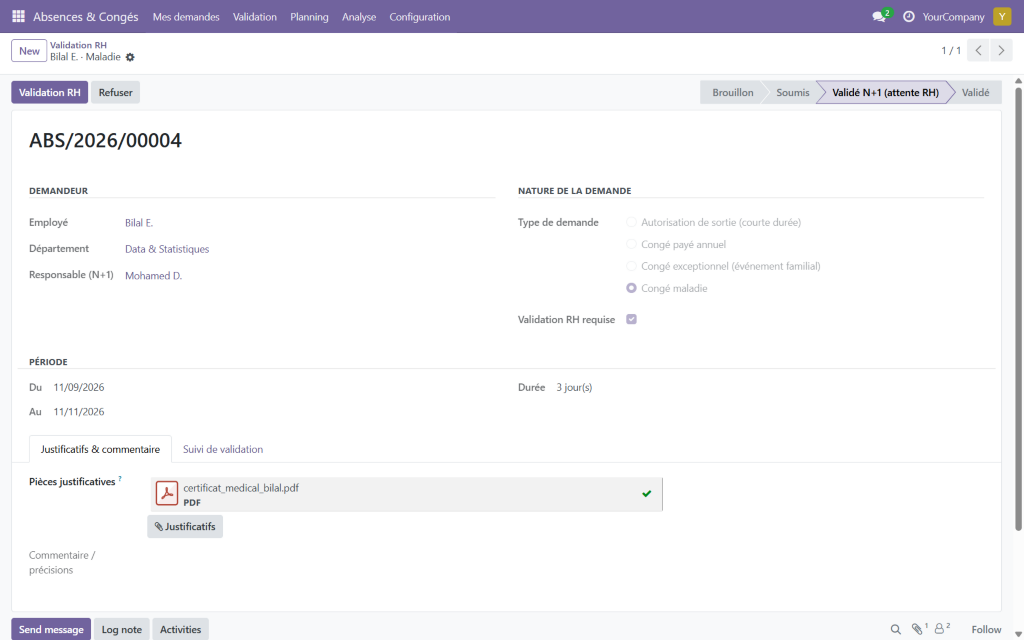
\includegraphics[width=0.95\textwidth]{figures/05_hr_validation.png}}
    \caption{Validation RH par Yahya G. du congé maladie de Bilal E. avec justificatif médical attaché}
    \label{fig:hr_val}
\end{figure}

Depuis \textit{Configuration $\rightarrow$ Soldes de congés} (figure~\ref{fig:hr_bal}), les RH pilotent les dates d'embauche, les reports/ajustements manuels et consultent en temps réel les compteurs acquis, pris, en attente et disponibles de chaque collaborateur. Enfin, le menu \textit{Analyse} (figure~\ref{fig:hr_ana}) fournit des vues Graphique et Tableau croisé dynamique sur les absences validées.

\begin{figure}[H]
    \centering
    \fbox{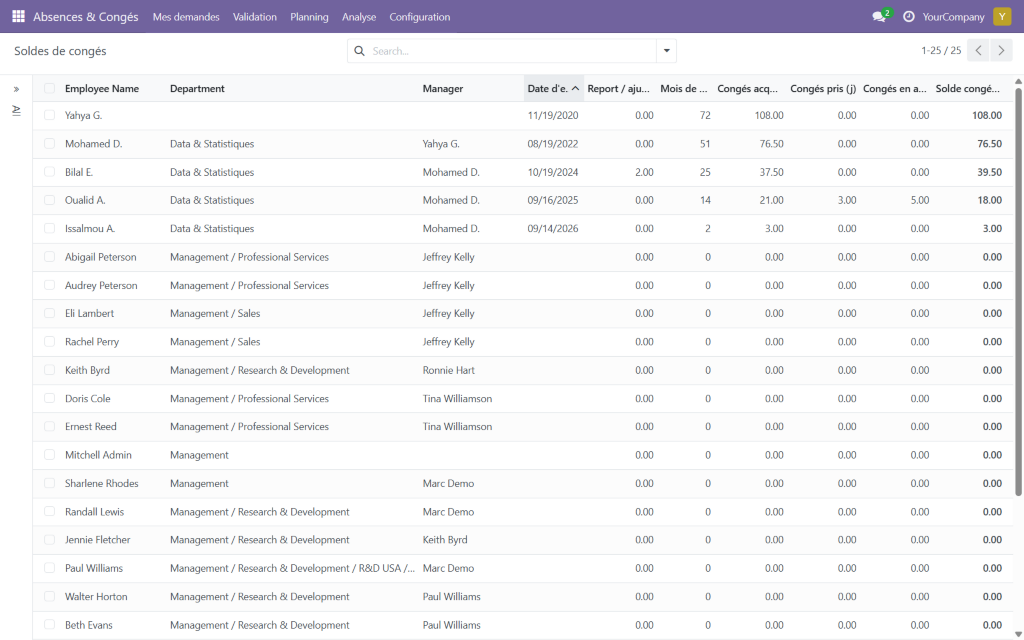
\includegraphics[width=0.95\textwidth]{figures/06_hr_balances.png}}
    \caption{Vue consolidée des soldes de congés payés (\textit{Configuration $\rightarrow$ Soldes de congés})}
    \label{fig:hr_bal}
\end{figure}

\begin{figure}[H]
    \centering
    \fbox{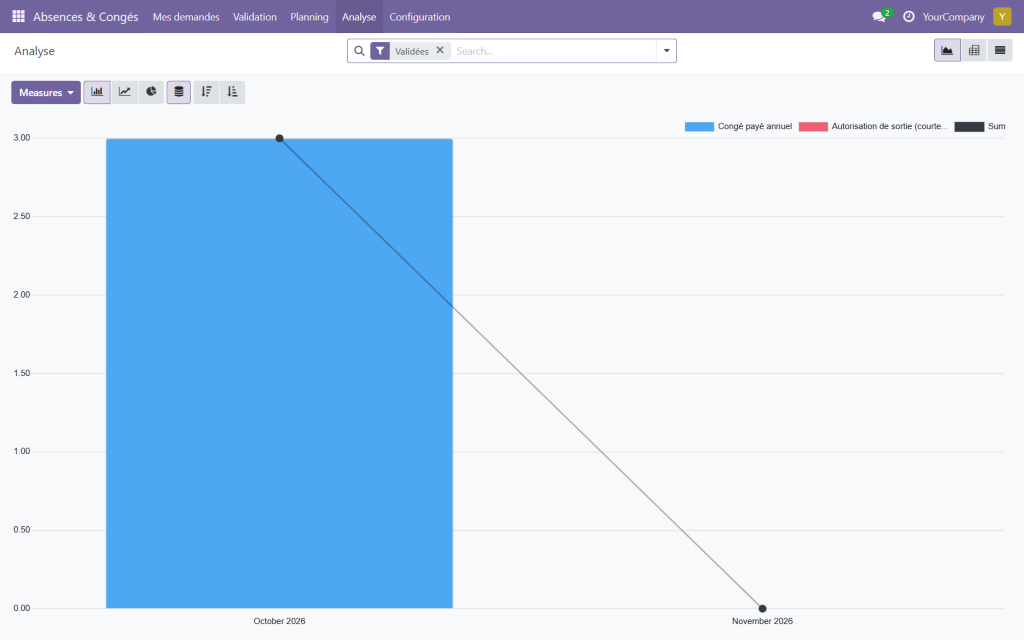
\includegraphics[width=0.95\textwidth]{figures/07_hr_analysis.png}}
    \caption{Tableau de bord analytique des absences validées (\textit{Analyse -- vue Graphique})}
    \label{fig:hr_ana}
\end{figure}

% =============================================================================
% 5. TESTS AUTOMATISÉS ET VALIDATION
% =============================================================================
\section{Tests Automatisés et Validation}

Afin de garantir la fiabilité de chaque règle de gestion, une suite complète de \textbf{25 tests automatisés} (\texttt{TransactionCase}) a été développée dans \texttt{tests/test\_absence\_request.py} et exécutée dans le conteneur Odoo 18 via la commande :
\begin{tcolorbox}[infobox, title={Commande d'exécution des tests automatisés}]
\small\texttt{docker compose exec -T odoo odoo -d insea\_db -i insea\_hr\_leave\_custom --test-enable --test-tags /insea\_hr\_leave\_custom --stop-after-init --db\_host db -r odoo -w odoo --http-port 8070}
\end{tcolorbox}

L'ensemble des tests s'exécute sans aucune anomalie : \textbf{\color{customBorder} 0 failed, 0 error(s) of 25 tests} (tableau~\ref{tab:tests}).

\begin{table}[H]
\centering
\caption{Couverture de la suite de tests automatisés (\texttt{TestAbsenceRequest})}
\label{tab:tests}
\small
\begin{tabularx}{\textwidth}{>{\bfseries}p{2.8cm} p{2.2cm} Y p{2.0cm}}
\toprule
Domaine testé & Tests & Règles vérifiées & Résultat \\
\midrule
Calculs \& calendrier & \texttt{test\_01} -- \texttt{02} & Acquisition 1,5 j/mois, déduction post-RH, exclusion week-ends et jours fériés. & \textbf{\color{customBorder} 2 / 2 OK} \\
Autorisations & \texttt{test\_03} -- \texttt{06} & Durée $\leq 4\text{ h}$, plafonds 3/mois et 8 h/mois, motif obligatoire, impact solde nul. & \textbf{\color{customBorder} 4 / 4 OK} \\
Contrôles métier & \texttt{test\_07} -- \texttt{11} & Non-chevauchement, solde insuffisant, réservation des demandes en attente, prévenance 7 j, durées familiales. & \textbf{\color{customBorder} 5 / 5 OK} \\
Circuit de validation & \texttt{test\_12} -- \texttt{21} & Validation finale N+1 (autorisation \& maladie 1 j), validation RH, blocage justificatif, assistant refus + notification, verrouillage post-soumission, interdiction d'auto-validation. & \textbf{\color{customBorder} 10 / 10 OK} \\
Sécurité \& SQL & \texttt{test\_22} -- \texttt{25} & Record Rules (Employé / Manager / RH), interdiction de créer pour un collègue, lecture du solde propre, contrainte SQL \texttt{check\_dates\_order}. & \textbf{\color{customBorder} 4 / 4 OK} \\
\midrule
\textbf{Total} & \textbf{25 tests} & \textbf{Couverture intégrale du cahier des charges} & \textbf{\color{customBorder} 25 / 25 OK} \\
\bottomrule
\end{tabularx}
\end{table}

% =============================================================================
% 6. CONCLUSION ET PERSPECTIVES
% =============================================================================
\section{Conclusion et Perspectives}

Le module \texttt{insea\_hr\_leave\_custom} répond intégralement aux besoins exprimés par la société \textbf{Lambda} pour la dématérialisation de ses autorisations d'absence et de ses congés. L'architecture retenue tire parti de la puissance du framework Odoo 18 (ORM, héritage par extension, mixins \texttt{mail}, sécurité multi-niveaux et vues analytiques) tout en assurant une maintenance propre et testée automatiquement.

En perspective d'évolution, le module pourrait être enrichi par :
\begin{itemize}[itemsep=2pt]
    \item l'export mensuel automatique vers un module de paie (Odoo Payroll) des absences validées ;
    \item l'ajout d'une délégation temporaire de validation en cas d'absence du manager N+1 ;
    \item la génération de rapports PDF individuels d'attestation de congé via QWeb.
\end{itemize}

\end{document}
